\chapter{QuickDough Design Framework} \label{chapter:framework}
QuickDough is a development framework for FPGA-accelerated applications. It generates FPGA accelerators for compute intensive loop kernels rapidly through the use of a pre-built soft coarse-grained reconfigurable array (SCGRA) overlay. QuickDough also performs application-specific customization and generates optimized SCGRA overlay as well as communication infrastructure between the CPU host and the accelerator automatically, integrating both software and hardware generation in a unified framework.

The overall design goal of QuickDough is to enhance the designer's productivity by greatly reducing the hardware generation time and by providing automatic optimization of the data I/O between the host software and the accelerator. Instead of spending hours on conventional hardware implementation tools, QuickDough is capable of producing the targeted hardware-software system in the order of seconds. By doing so, it provides a rapid development experience that is compatible with that expected by most software programmers.

To achieve this compilation speed, while maintaining a reasonable accelerator performance, QuickDough avoids the creation of custom hardware directly for each application. Instead, the compute kernel loop bodies are scheduled to execute on a CGRA overlay, which is selected from a pre-implemented CGRA based accelerator library. By sidestepping the time-consuming low-level hardware implementation tool flow, the time to implementing an accelerator in QuickDough is reduced to essentially just the time spent on overlay selection and scheduling compute operations on the resulting overlay. In addition, taking advantage of the overlay's softness and regularity, QuickDough allows users to perform trade-off between compilation time and performance by selecting and customizing the overlay on a per application basis. The result is a unified design framework that seamlessly produces the entire hardware-software infrastructure with a design experience similar to developing conventional software.

This chapter mainly focuses on the the basic compilation flow from high-level loop kernels to the SCGRA overlay based FPGA accelerator bitstream and it will be organized as follows. The overall QuickDough design framework will be presented in the next section. The processes in the rapid QuickDough compilation flow will be detailed in \secref{sec:loop-compilation}. Finally, the accelerator library used in the rapid compilation flow as well as its pre-building process will be explained in \secref{sec:library-update}.    

\section{QuickDough Overview}
\figref{fig:framework} summarizes the hardware-software compilation flow of QuickDough. Users begin by specifying the regions for accelerations in the form of compute intensive loops. Once a loop is identified, it is further compiled to an SCGRA overlay based FPGA accelerator through SCGRA customization and SCGRA compilation while the rest part of the program is compiled to the processor through a conventional software compilation.

\begin{figure}
    \center{\includegraphics[width=0.7\linewidth]{framework}}
    \caption{QuickDough: FPGA Loop Accelerator Design Framework Using SCGRA Overlay.}
    \label{fig:framework}
\end{figure}

QuickDough partitions the complex SCGRA overlay based accelerator development flow into two paths. Along the rapid and common acceleration generation path, QuickDough first translates the compute-intensive loop kernels into data flow graphs (DFGs) and then statically schedules the DFGs on to the SCGRA overlay. Afterwards, it integrates the scheduling result with a partially implemented overlay bitstream which is selected from a pre-built overlay based accelerator bitstream library. By employing different selection algorithms on the accelerator library, QuickDough allows users to perform trade-off between performance and compilation time. At the end of the selection process, optimized communication interfaces will be generated accordingly.

QuickDough also includes a relatively slow yet less frequent accelerator library update path which pre-build the SCGRA overlay based accelerator library. To expedite the library generation process, a small representative set of accelerator configurations are chosen as the library and generated automatically using an SCGRA overlay template based system. Although it does take some time to build the accelerator library, the library can be reused during design iterations of an application or shared by a domain of applications and thus the library building time can be amortized. In addition, the SCGRA overlay template is highly pipelined to allow high-frequency and high-performance overlay based accelerator implementation. The SCGRA overlay is also regular and scalable, which makes the resulting accelerators conveient to be adapted to different applications.  

In addition, QuickDough supports automatic application-specific customization all the way from high level loop unrolling, on-chip buffer sizing and overlay structure configuration to achieve optimized performance and energy efficiency of the resulting accelerator. The automatic customization process helps the users to explore the large and complex design space and it also makes QuickDough accessible to software designers. The customization process introduces moderate time consumption, but it is optional and the customized accelerator configuration can also be added to the accelerator library for reuse in future. Detailed customization process will be presented in next chapter.

The slow path of QuickDough is to update the accelerator library upon users' request and users may simply provide the hardware resource budget. Then target operations to be supported will be decided automatically by analyzing the DFGs produced by the DFG generator. With the resource budget and the supported operation set, a set of representative accelerator HDL models will be generated by utilizing the overlay based accelerator template. Finally, the accelerator HDL models are implemented on the target FPGA platform and further added to the accelerator library.

\section{Rapid Accelerator Generation} \label{sec:loop-compilation}
The rapid acceleration generation path of QuickDough consists of a series of inter-related steps as illustrated in \figref{fig:framework}. In the first step, the compute intensive loop kernel is statically transformed to the corresponding data flow graph (DFG) with specified loop unrolling factor which can either be user input or be obtained from the customization process. Then the accelerator selection process selects an accelerator from a pre-built accelerator library based on the scheduling performance and the communication cost. The scheduling performance is obtained from the SCGRA scheduling process which schedules the generated DFG to the SCGRA overlay included in the selected accelerator while the communication cost is obtained through a CPU-FPGA communication estimation model. After the accelerator selection process, the accelerator drivers can be generated accordingly based on the on-chip buffer size of the selected accelerator. Meanwhile, the selected empty pre-built accelerator bitstream and the corresponding scheduling result are integrated to create the final FPGA accelerator configuration bitstream. This bitstream, in combination with the binary code created in the software compilation process, forms the final application that will be executed on the target CPU-FPGA system.

\subsection{DFG Generation and Loop Execution}
The main input to the QuickDough framework for acceleration are compute intensive kernels extracted from the user applications. The first step of the compilation process is therefore to extract data flow graphs (DFGs) from these kernels that are often expressed as inner loop bodies. In order to express the loop bodies as DFGs, data dependency in the loop body must be known at compilation time. Similar to LLVM intermediate representation \cite{llvm}, branches in the loop bodies can be removed by using PHI instructions which can be further mapped to the PHI operation as described in previous chapter. While this strategy helps to extend the reach of the SCGRA overlay based loop acceleration, it remains challenging to convert large and complex branches. In this work, a C++ library is built to help automate the DFG generation with specified operation set and loop unrolling.

The loop kernels are partially unrolled, transformed to DFGs and scheduled to the SCGRA overlays of the accelerators. A straightforward way to perform the whole loop computation on the overlay is to repeat the same DFG computation until the end of the loop. Nevertheless, this may require data transfer between host processor and I/O buffer for each DFG computation. As a result, the communication cost increases dramatically especially when the amount of each data transfer is small. Worse still, input data of the consecutive DFGs may be reused and the straightforward data transfer strategy may greatly increase the total amount of data transfer through out the loop computation. 

To alleviate this problem, we have proposed to batch data transfers for multiple executions of the same DFG into groups as shown in \figref{fig:blocking-and-dfg-gen}. Specifically, after the loop is unrolled $U$ times, $G$ of them are grouped together for each data transfer. This group strategy helps to amortize the initial communication cost between host processor and the accelerator. In addition, it allows input data to be reused for different DFG computation in the same group and the group size is mainly limited by the I/O buffer depth. Meanwhile, the accelerator communicates with host processor for each group execution, and thus the accelerator driver that handles the communication depends on the I/O buffer depth as well. 

While grouping data transfers helps amortize the communication cost between CPU and the accelerator, it also imposes additional requirement for on-chip memory to serve as buffer for the extra data transferred. As a result, the unrolling factor $U$ and grouping factor $G$ has to be co-optimized to balance performance and on-chip resource utilization. For instance, increasing $U$ leads to a larger DFG to be executed in the QuickDough overlay, which may be benefited from a larger processing array. However, the increased processing array limits the amount of on-chip buffer available for data and address buffer. As a result, the amount of DFG grouping $G$ is limited and may lead to higher performance penalty due to communication. In addition, the proposed accelerator employs address buffers to store all the on chip buffer accessing addresses of the whole group execution. While the addresses of different DFG execution in a group can't be reused, the capacity of the address buffers is the product of the number of input/output addresses of a DFG and the number of DFGs in a group, which is usually larger than the capacity of the input/output buffers especially when there are a large amount of input/output data reuse between different DFGs in the same group. 

\begin{figure}
\center{\includegraphics[width=0.75\linewidth]{dfg-gen}}
\caption{Loop execution on an SCGRA overlay based FPGA accelerator}
\label{fig:blocking-and-dfg-gen}
\end{figure}

\subsection{DFG Scheduling}
The operations from the user DFG are scheduled to execute on the reconfigurable array. Since the processing elements in the QuickDough overlay execute in lock steps with deterministic latencies, a classical list scheduling algorithm \cite{schutten1996list} was adopted. The challenge in this scheduler is that data communication among the processing elements must be carried out via multi-hop routing in the array. As a result, while it is desirable to schedule data producers and consumers in nearby processing elements to minimize communication latencies, it is also necessary to utilize as much parallel processing power as possible for sake of load balancing. Building on top of our previous work presented in \cite{lin2012energy}, a scheduling metric considering both load balancing and communication cost was adopted in our current implementation.

 \begin{algorithm}
 \small
 \caption{The QuickDough scheduling algorithm.}
 \label{alg:scheduling}
 \begin{algorithmic}
 \PROCEDURE{ListScheduling}
 \STATE Initialize the operation ready list $L$
 \WHILE {$L$ is not empty}
 \STATE select a PE $p$ with lowest utilization
 \STATE select an operation $l$ that completes computing earliest
 \STATE OPScheduling($p$, $l$)
 \STATE Update $L$
 \ENDWHILE
 \ENDPROCEDURE
 \STATE
 \PROCEDURE {OPScheduling($p$,$l$)}
 \FORALL {predecessor operations $s$ of $l$}
 \STATE Find nearest PE $q$ that has a copy of operation $s$
 \STATE Find shortest routing path from PE $q$ to PE $p$
 \STATE Move operation $s$ from PE $q$ to PE $p$ along the path
 \ENDFOR
 \STATE Do operation $l$ on PE $p$
 \ENDPROCEDURE

 \end{algorithmic}
 \end{algorithm}

\algref{alg:scheduling} briefly illustrates the scheduling algorithm implemented in QuickDough. Initially, an operation ready list is created to represent all operations that are ready to be scheduled. The next step is to select a PE from the SCGRA and an operation from the ready list using a combined communication and load balance metric. Basically the PE with lowest utilization is choosen as the target processing element for the next operation. Then estimate the execution time of all the ready operations on the selected PE. The operation that completes computing earliest will be selected and scheduled. When both the PE and the operation to be scheduled are determined, the \code{OPScheduling} procedure starts. It determines an optimized routing path, moves the source operands to the selected PE along the path, and schedules the selected operation to execute accordingly. After this step, the ready list is updated as the latest scheduling may produce more ready operations. This \code{OPScheduling} procedure is repeated until the ready list is empty. Finally, given the operation schedule, the corresponding control words for each PE and the IO buffer accessing sequence will be produced. These control words will subsequently be used for bitstream generation in the following compilation step.

\subsection{Accelerator Selection} \label{sec:accel-sel}
Accelerator selection process selects an accelerator from the accelerator library based on the performance of the resulting accelerator which mainly depends on the computation latency and communication latency. The computation latency of the loop kernel can be calculated using \eqnref{eq:comp-lat}. $DFG\_Lat$ stands for the number of cycles needed to complete the SCGRA scheduling and mostly depends on the SCGRA overlay size while $Freq$ stands for the pre-built accelerator implementation frequency. The communication latency can be calculated using \eqref{eq:comm-lat} where $Trans()$ represents the data transfer latency function of the target platform and $GpIn$ and $GpOut$ represent the amount of data transfer of a group which is limited by the capacity of the I/O buffers. 

\begin{equation} \label{eq:comp-lat}
    \footnotesize
    CompLat = DFG\_per\_Loop \times DFG\_Lat / Freq
\end{equation}


\begin{equation} \label{eq:comm-lat}
    \footnotesize
    CommLat = Gp\_per\_Loop \times (Trans(GpIn) + Trans(GpOut))
\end{equation}


In summary, the performance of the accelerator can be estimated with analytical models when the scheduling performance is obtained through the DFG scheduling while the scheduling performance is mostly determined by the SCGRA overlay size. The analytical estimation is fast while the scheduling process is relatively slow. Therefore, the accelerator selection process essentially centers the SCGRA overlay size selection and then explores all the accelerator configurations (such as on chip buffer size, instruction memory depth and data memory size) with the same SCGRA overlay size. 

To compromise the loop accelerator generation time and performance, three different levels of accelerator selection optimization levels are provided in this framework namely O0, O1 and O2 centering the SCGRA overlay size selection. O0 doesn't provide any optimization, and it selects an accelerator with the smallest SCGRA overlay. O1 estimates three typical accelerators with the smallest SCGRA overlay, a medium one and the largest SCGRA overlay. Then the one that provides the best performance will be adopted. O2 explores all the accelerators in the library and searches for the best accelerator configuration. With the increase of the optimization level, the accelerator selection process spends more effort in searching the accelerator library for better performance and thus results in longer compilation time.

\subsection{Bitstream Integration}
The final step of the compilation is to generate the instructions for each PE and the address sequences for the I/O buffers according to the scheduler's result, which will subsequently be incorporated into the configuration bitstream of the overlay produced from previous steps.
By design, our overlay does not have any mechanism to load instruction streams from external memory.
Instead, we take advantage of the reconfigurability of SRAM based FPGAs and store the cycle-by-cycle configuration words using on-chip ROMs. The content of the ROMs are embedded in the bitstream and the \code{data2mem} tool from Xilinx \cite{data2mem} is used to update the ROM content of the pre-built bitstream directly. To complete the bitstream integration, \code{BMM} file that describes the organization and placements of the ROMs in the overlay is extracted from \code{XDL} file corresponding to the overlay implementation \cite{beckhoff2011xilinx}.
This bitstream integration process costs only a few seconds of the compilation time.

\section{Accelerator Library Update} \label{sec:library-update}
The accelerator library consists of a number of pre-built SCGRA overlay based accelerators with different configurations. It is the basis for the proposed rapid FPGA loop accelerator generation framework. In this section, we will illustrate how the accelerator library is updated given the hardware resource budget and target loop kernels.

An accelerator library update is essentially to pre-implement a group of SCGRA overlay based FPGA accelerators upon the users' request, which may either target a specified application or a domain of applications. As QuickDough aims to enhance the designers' productivity and make FPGA accelerator design accessible to high-level application designers, the library update which involves low-level circuit design and optimization is thus automated so that it will not become a new barrier to the application developer.

\figref{fig:auto-lib-gen} presents the proposed automatic accelerator library update flow. It roughly consists of four steps i.e. DFG generation, common operation analysis, minimum accelerator configuration set analysis, and accelerator HDL model generation and implementation. Since DFG generation has been discussed in previous section, we will mainly detail the remaining three steps in this section.

\begin{figure}
\center{\includegraphics[width=0.8\linewidth]{lib-gen}}
\caption{Automatic SCGRA overlay based FPGA accelerator library update}
\label{fig:auto-lib-gen}
\end{figure}

\subsection{Common Operation Analysis}
In this framework, the operations used to construct the DFG is up to the DFG generation process and the common operation analysis step mainly decides the minimum operation set that is needed to support the target applications. It is possible to co-optimize the DFG generation and common operation set analysis, but it is beyond the discussion of this work. Currently, we just perform a union of the operation types included in the DFGs. It is trivial, but the minimum operation set can be decided automatically and rapidly.

\subsection{Minimum Accelerator Configuration Set Analysis}
Although the library can be implemented off-line, it does take a long time to complete.
Therefore, we try to find out the minimum set of accelerator configurations that need to be
pre-implemented as the library and maintain the application coverage of the library at the same
time. 

The proposed SCGRA overlay based FPGA accelerator utilizes
block RAM to implement the instruction memory, data memory, on-chip buffer as well as the address
buffer. As a result, the block RAM becomes the hardware resource bottleneck and the library basically depends on how
the block RAM budget is allocated to different components of the accelerators. Therefore, the
minimum library can be obtained using equation \eqnref{eq:lib-gen}. $Row$ and $Col$ stand for the SCGRA
overlay size and they are integers. $IM$, $DM$, $AIOB$ and $DIOB$ stand for the instruction memory capacity,
data memory capacity, address IO buffer capacity and IO buffer capacity. In addition, they can only increase with the granularity of a primitive block RAM. $B$ stands for the user specified block RAM budget. 

\begin{equation} \label{eq:lib-gen}
    \footnotesize
    Row \times Col \times(IM + DM) + AIOB + IOB \leq B
\end{equation}

Moreover, empirical settings such as limiting data memory in each PE to a single primitive block RAM
(i.e. $DM = 1$), constraining the difference between SCGRA row size and column size (i.e. $Col \leq
Row \leq (Col + Gap)$, $Gap$ is an integer) and setting $AIOB = IOB$ are employed to further reduce the number of
accelerators pre-built in the library.  

\subsection{Accelerator HDL Model Generation and Implementation}
The QuickDough overlay is a highly regular processing array that can be generated easily according to the template as described in previous chapter. The overlay may be customized in many aspects, including the type of operation supported by each processing element (PE), the processing array size, its topology, as well as the number and capacity of the data buffers. With the proposed SCGRA overlay template and the accelerator configurations to be pre-built in the library, corresponding HDL models of the SCGRA overlay based FPGA accelerators are generated with a python script. Then the library can be implemented using the conventional hardware implementation tools. The lengthy implementations can be done in parallel. Moreover, the regular tiling structure even allows the implementations to be accelerated using macro based implementation techniques as presented in \cite{yue2015rapid}, which can be up to 20X faster than a standard HDL implementation with negligible timing and overhead penalty. After the implementation, implementation frequency is added to the corresponding accelerator configuration, which completes the whole library update process.

\section{Experiments}
With an objective to improve designers' productivity in developing FPGA accelerators, the key goal of QuickDough is to reduce FPGA loop accelerator development time for a hybrid CPU-FPGA system. By using four typical loop kernels as the benchmark, we have evaluated the FPGA accelerator generation time with QuickDough. Meanwhile, to warrant the merit of such framework, the performance of the generated acceleration system should remain competitive. For that purpose, the performance is then compared against to that of software executed on an ARM processor. Finally, the pre-built accelerator library that affects both the design productivity and overhead of the resulting accelerators is also
discussed.

%The experiment section is organized as follows. We will first briefly introduce the benchmark programs in the following subsection and explain the basic experiment setup in \secref{subsec:setup}. Then we will discuss the accelerator library update in \secref{subsec:lib-update}. Finally, we will elaborate the loop accelerator generation time, performance and implementation overhead in \secref{subsec:acc-gen}, \secref{subsec:acc-perf} and \secref{subsec:acc-impl} respectively. 

\subsection{Benchmark} \label{subsec:benchmark}
Four applications were used as benchmark in this work, namely, a matrix-matrix multiplication (MM), a finite impulse response (FIR) filter, a K-mean clustering algorithm (KM) and a Sobel edge detector (SE). The basic parameters and configurations of the benchmark are illustrated in \tabref{tab:benchmark-config}. 

\begin{table}[htb]
    \footnotesize
    \centering
    \caption{Detailed Configurations of the Benchmark 
    \label{tab:benchmark-config}}{
        \centering
            \begin{tabular}{l|l|l|l}
                \hline
                MM & FIR & SE & KM \\ \hline
                Matrix Size & \tabincell{l}{\# of Input/ \\ \# of Taps+1} & \tabincell{l}{ \# of Vertical Pixels/ \\ \# of Horizontal Pixels} & \tabincell{l}{\# of Nodes/Centroids/ \\ Dimension} \\ \hline
                100 & 10000/50 & 128/128 & 5000/4/2  \\ \hline
            \end{tabular}
        }
\end{table}

\subsection{Experiment Setup} \label{subsec:setup}
The Xilinx implementation tools were run on a computer with Intel Core i5-3230M CPU and \SI{8}{\giga\byte} of RAM. The resulting HW-SW Co-design was targeted at Zedboard with both a hard ARM processor and an XC7Z020 FPGA. Software runtime was obtained from the ARM processor with -O3 compiling option. The accelerators were implemented on the FPGA of Zedboard. ISE 14.7 was used to implement the overlay based FPGA accelerators. 

The acceleration system handles the input data loading, accelerator computation and output data storing sequentially. The performance of the accelerators is calculated using \eqnref{eq:comp-lat} and \eqnref{eq:comm-lat} in \secref{sec:accel-sel}. The data transfer latency used in \eqnref{eq:comm-lat} is estimated based on Zedboard DMA between main memory and FPGA on-chip buffer through AXI high-performance port. The transfer latency is detailed in \tabref{tab:latency}. When the transfer size is not included in the table, a simple linear model is used to estimate its latency. Fmax and the number of cycles were extracted from the ISE14.7 and SCGRA scheduler respectively. 
 
\begin{table}
\footnotesize
    \centering
    \caption{DMA transfer latency on Zedboard through AXI high performance port \label{tab:latency}}{
        \centering
            \begin{tabular}{c|c|c|c|c|c|c|c}
                \hline
                \tabincell{c}{transfer \\ size (word, 32bit)} & $\geq$512 & 256 & 128 & 64 & 32
                                                                  & 16 & $\leq$8  \\ \hline
                \tabincell{c}{Latency per \\ word (ns)}  & 10.08 & 11.28 & 13.32 & 15.18 & 21.45 & 36.24 & 63 \\ \hline
            \end{tabular}
        }
\end{table}

Loop unrolling is a critical design input parameter for FPGA loop accelerators developed using QuickDough. It determines the parallelism that are exposed to the overlay architecture and influences the accelerator selection. While tuning the major accelerator design parameters together helps to achieve an optimized loop accelerator design, it requires more design efforts as to be detailed in \chapref{chapter:customization}. \tabref{tab:unrolling-setup} shows the loop unrolling factors that are used for the loop accelerator generation.

\begin{table}
\footnotesize
\centering
\caption{QuickDough unrolling setup \label{tab:unrolling-setup}}{
        \begin{tabular}{l|l|l|l|l}
            \hline
           & MM & FIR & SE & KM \\ \hline
            Unrolling & $1 \times 5 \times 100$ & $50 \times 50$ & $16 \times 16 \times 3 \times 3$ &
            $125\times 4 \times 2$ \\ \hline
            DFG size & 750 & 2500 & 9720 & 5768 \\ \hline
            Full Loop & $100 \times 100 \times 100$ &  $10000 \times 50$ & $128 \times 128 \times 3
            \times 3$ & $5000 \times 4 \times 2$ \\ \hline
        \end{tabular}
}
\end{table}

\subsection{Accelerator Library Update} \label{subsec:lib-update}
To ensure a rapid FPGA accelerator generation, we have implemented a group of 
SCGRAs based accelerators as the pre-built library by using the SCGRA overlay template. 
The library is developed to support all the four loop kernels, and it includes 12 
3-source-1-destination operations as presented in previous chapter. 

In addition, empirical settings are adopted to reduce the number of accelerators to be built in
library. Input and output buffer depth are set to be the same. The depth of the address buffers are
set to be twice with that of the I/O buffer depth. The data memory in each PE consumes only one
primitive block RAM. Instruction memory depth and I/O buffer depth are set to be $2^n$K $(n=0,1,2,
...)$. The SCGRA overlay adopts a torus topology, and the row size is set to be equal
to the column size or larger by one for the sake of performance. Eventually, different accelerator
configurations mainly differ on the on-chip I/O buffer depth, SCGRA size and instruction memory depth
when the data width is determined. 

To explore the library update process efficiency, we have evaluated the number of accelerators included in
the accelerator library and the time consumed to implement the library when different block RAM
budgets ranging from 70, 140, 210, 280 to 350 RABM36 (Note that there are 140 RAMB36 on Zedboard FPGA) are
provided. As presented in \figref{fig:lib-impl-time}, when the BRAM budget increases, the number of accelerators
in the library and the library implementation time increase almost linearly. With a single
computer, the accelerator library implementation time ranges from 164 minutes to 3035 minutes.
However, with a cluster, the time cost of the highly parallel library implementation can decrease by
an order of magnitude easily.

\begin{figure}
\centering
\includegraphics[width=0.6\linewidth]{lib-impl-time}
\caption{Accelerator library size and implementation time given different BRAM budgets.}
\label{fig:lib-impl-time}
\end{figure}

\subsection{Accelerator Generation Time} \label{subsec:acc-gen}
In this section, the loop accelerator generation time of QuickDough is evaluated. 
It is used as an indicator on the designer's productivity as it greatly limits 
the number of compile-debug-edit cycles achievable per day. 

In order to evaluate the loop accelerator generation time, we took the FPGA resource on Zedboard as
the resource budget and pre-built the accelerator library.
Then FPGA loop accelerators were generated for each application in the benchmark using the three
different accelerator selection options i.e. O0, O1 and O2.  
\tabref{tab:final-acc-config} shows the configurations of the resulting
FPGA accelerators as well as corresponding grouping factors. 

\begin{table}
\footnotesize
\centering
\caption{Accelerators generated using QuickDough \label{tab:final-acc-config}}{
        \begin{tabular}{l|l|l|l|l|l}
            \hline
            \tabincell{c}{Opt. \\ option} & \tabincell{c}{Resulting \\ Config.} & MM & FIR & SE & KM \\ \hline
            \multirow{3}{*}{O0}  & SCGRA size & $2 \times 2$ & $2 \times 2$ & $2 \times 2$ & $2 \times 2$ \\ \cline{2-6} 
                                & Inst. Mem depth & 4K  & 4K & 4K & 4K \\ \cline{2-6} 
                                & I/O buffer depth & 4K & 4K & 4K & 4K \\ \cline{2-6}
                                & Grouping factor & 50x5x100 & 2500x50 & 128x64x3x3 & 1250x4x2 \\ \hline
            \multirow{3}{*}{O1}  & SCGRA size & $3 \times 3$  & $3 \times 3$  & $3 \times 3$  & $5
            \times 5$  \\ \cline{2-6} 
                                & Inst. Mem depth & 2K & 2K & 4K & 1K \\ \cline{2-6} 
                                & I/O buffer depth & 2K & 2K & 1K & 2K \\ \cline{2-6}
                                & Grouping factor & 25x5x100 & 1250x50 & 64x32x3x3 & 1000x4x2\\ \hline
            \multirow{3}{*}{O2}  & SCGRA size & $3 \times 3$ & $4 \times 4$  & $4 \times 4$  & $5
            \times 5$  \\ \cline{2-6} 
                                & Inst. Mem depth & 2K & 1K & 2K & 1K \\ \cline{2-6} 
                                & I/O buffer depth & 2K & 8K & 1K & 2K \\ \cline{2-6} 
                                & Grouping factor & 25x5x100 & 5000x50 & 64x32x3x3 & 1000x4x2 \\ \hline

        \end{tabular}
    }
\end{table}

With the pre-built library, every implementation iteration in QuickDough involves 3 steps:
\begin{itemize}
\item DFG generation: The compute kernel is translated to corresponding DFG.
\item Accelerator selection and DFG scheduling: Select an accelerator configuration and schedule the DFG to it through an operation scheduling. 
\item Bitstream generation: The scheduling result is embedded into a pre-built accelerator bitstream 
to produce the final FPGA bitstream of the compute kernel.
\end{itemize}

\figref{fig:SCGRA-Overlay-Compilation-Time} shows loop accelerator generation time of QuickDough.
Both DFG generation and bitstream integration are very fast compared to the DFG scheduling step. The DFG
scheduling is relatively slower, but it usually completes in a few seconds.
Since the DFG scheduling process must be repeated when QuickDough explores different SCGRA size in
the accelerator library, the time consumption increases accordingly. Typically, the accelerator
generation time is relatively longer for more intensive accelerator selection. With O0 selection
where only a single DFG scheduling process targeting 2x2 SCGRA is needed, the accelerator can be
produced in less than 10 seconds. With O1 selection where three typical size of SCGRA (i.e. 2x2,
3x3, 5x5) will be evaluated, the accelerator
generation process completes in around half a minute. With the O2 selection where an exhaustive
search is performed, there are 76 accelerator configurations but only 7 different types of SCGRA
size are included in the library. 7 DFG scheduling processes are needed and the accelerator is
generated in one or two minutes.

\begin{figure}
\centering
\includegraphics[width=0.8\linewidth]{quickdough-runtime}
\caption{Time Consumption of Loop Accelerator Generation Using QuickDough.}
\label{fig:SCGRA-Overlay-Compilation-Time}
\end{figure}

Clearly, the designer must spend the time to physically pre-implement the overlay architecture on the target FPGA, spending considerable time on the implementation tools. However, it can be reused by the whole benchmark. Moreover, the designer may iterate via the above rapid steps during design and debugging phases using an initial overlay implementation. Once the functionality is frozen, the designer may then opt to further optimize performance through more intensive overlay customization and update the library. We argue that the ability to separate functionality and optimization concern, and the possibility of performing rapid debug-edit-implement iterations in QuickDough are crucial factors that contribute to a high-productivity design experience.

\subsection{Performance} \label{subsec:acc-perf}
While improving designers' productivity is the primary goal of QuickDough, the FPGA accelerators that it generates must remain competitive in terms of performance when compared to corresponding software executed on general purposed processors. Therefore, execution time of the loop kernels executed on ARM processor of Zedboard and FPGA accelerators generated using QuickDough are compared.

\figref{fig:real-perf} shows the accelerator performance speedup over software execution on the ARM processor and execution time decomposition of the 4 benchmark programs. The reported loop execution time on the accelerators includes time spent on I/O data communication between FPGA and the ARM processor as well as FPGA computation.

\begin{figure}
\centering
\subfigure[MM]{
\label{fig:mm-real-perf}
\includegraphics[width=0.44\linewidth]{mm-perf}}
\qquad
\subfigure[FIR]{
\label{fig:fir-real-perf}
\includegraphics[width=0.44\linewidth]{fir-perf}}
\qquad
\subfigure[SE]{
\label{fig:sobel-real-perf}
\includegraphics[width=0.44\linewidth]{se-perf}}
\qquad
\subfigure[KM]{
\label{fig:kmean-real-perf}
\includegraphics[width=0.44\linewidth]{km-perf}}
\caption{Benchmark performance speedup over software executed on ARM processor and execution time 
    decomposition of loop accelerators generated using QuickDough.}
\label{fig:real-perf}
\end{figure}

The results in \figref{fig:real-perf} show that the accelerators generated using QuickDough are 
capable to provide up to 9X performance speedup over software executed on ARM processor. For FIR, SE 
as well as KM which have abundant parallelism and moderate I/O requirements, the maximum speedup
goes up to 9X, 6X and 6X respectively. Even with simple acceleration selection and smallest SCGRA
size, clear performance speedup can be observed. MM optimized by simple loop unrolling is eventually reduced to
a matrix-vector multiplication, so the compute kernel has low compute-to-IO rate and the single port
connection between compute logic and input/output buffers becomes the bottleneck hindering
the performance of the accelerator. (Note that the communication time in \figref{fig:real-perf} simply shows the data movement time from/to main memory to/from accelerator IO buffers, it is NOT a sign of compute-to-IO rate. Usually, we may use operations per IO as the metric of compute-to-IO while IO indicates the load/store from/in input/output buffers.)

Accelerators with larger SCGRA overlay size typically achieve better performance than the ones with smaller overlay size. However, larger SCGRA overlay will not always guarantee better performance. As shown in the experiments, the largest $5 \times 5$ SCGRA overlay based accelerator is only optimal for KM. There are a few reasons for such an accelerator selection. First of all, accelerators with larger overlay size consume 
more block RAM for instruction memory leaving less block RAM for I/O buffer. As a result, the I/O
buffer may limit the transfer size between main memory and FPGA on-chip I/O buffer and reduce the
chance of data reuse between DFGs included in a single group. This increased number of transfer
between main memory and FPGA significantly limits the overall performance accordingly. Secondly, 
accelerator with larger SCGRA overlay may confront scheduling problem as larger SCGRA
overlay requires larger average cost between PEs and the compute performance may degrade as well.
Finally, larger SCGRA overlay based FPGA accelerators may result in lower implementation frequency
and degrade the overall performance as well. Optimal accelerators have the best trade-off on
buffering, scheduling and implementation frequency. According to \figref{fig:real-perf}, 3x3 or 4x4
SCGRA based FPGA accelerator achieve relatively better performance.

\subsection{Implementation Frequency and Hardware Overhead} \label{subsec:acc-impl}
One advantage of employing a simple and regular overlay architecture allows highly 
pipelined implementations with much higher frequencies as shown in \figref{fig:impl-freq}. 
The increased running frequency in turns results in higher overall 
performance of the system. Though both larger SCGRA overlay size 
and deeper instruction memory may degrade the implementation frequency, the FMax of the
implementations is typically around 250MHz on Zedboard FPGA which is much higher than random logic
synthesis on Zedboard.

\begin{figure}[htb]
\center{\includegraphics[width=0.65\linewidth]{impl-freq}}
\caption{fmax of The Accelerators Generated Using QuickDough}
\label{fig:impl-freq}
\end{figure}

As presented in \figref{fig:hw-overhead}, block RAM is the resource bottleneck for the SCGRA overlay
based FPGA accelerators. It may result in lower implementation frequency as the high utilization may
cause tight placing and routing. LUT, FF and DSP48 overhead mainly depends on the SCGRA overlay size and only a
portion of them are utilized.

\begin{figure}[htb]
\vspace{1em}
\center{\includegraphics[width=0.8\linewidth]{hw-overhead}}
\caption{FPGA Accelerator Recource Utilization}
\label{fig:hw-overhead}
\end{figure}

\section{Summary}
In this work, the QuickDough compilation framework for high productivity development of FPGA-based accelerators is presented. QuickDough makes use of a soft coarse-grained reconfigurable array as an overlay architecture to greatly improve the designer's compilation experience. Taking advantage of a pre-built SCGRA overlay based accelerator libray, the lengthy low-level FPGA accelerator implementation is reduced to a rapid operation scheduling problem and the compilation time of QuickDough is reduced to seconds, which contributes directly into higher application designers' productivity. Despite the use of an additional layer of overlay architecture on the target FPGA, the overall application performance remains competitive in many cases.
